\documentclass[11pt,a4paper]{scrartcl}
\usepackage[czech]{babel}
\usepackage[utf8]{inputenc}
\usepackage{graphicx}
\usepackage{float}

\begin{document}
	\title{Semestrální práce z předmětu KIV/PPR}
	\subtitle{Prolomení šifry SkipJack}
	\author{Zdeněk Valeš}
	\date{22.11. 2018}
	\maketitle
	\newpage
	
	\section{Zadání}
	Vaším úkolem bude prolomit šifru SkipJack. Tuto šifru je výpočetně náročné prolomit hrubou silou, nicméně lze zkusit i sofistikovanější metody např. genetické a evoluční algoritmy. Abyste prolomení urychlili, lze referenční kód přepsat a vektorizovat na úrovni instrukcí, pomocí GPU, případně ho distribuovat pomocí MPI.
	
	Samostatná práce využije alespoň dvě z celkem tří možných technologií:
	
	\begin{itemize}
		\item Paralelní program pro systém se sdílenou pamětí - C++, popř. WinAPI
		\item Program využívající asymetrický multiprocesor - konkrétně x86 CPU a OpenCL kompatibilní GPGPU - C++ AMP
		\item Paralelní program pro systém s distribuovanou pamětí - C++ MPI
	\end{itemize}

	Práci implementujte v jazyce C++ do základu aplikace, který je k dispozici na CourseWare.
	
	\section{Popis řešení}
	Vstupem prolamovací funkce je zašifrovaný blok a referenční blok. Cílem algoritmu je nalezení klíče (jedince) po jehož použití v dešifrovací funkci bude vstupní blok identický s referenčním. Algoritmus je znázorněn na obrázku \ref{fig:alg}.
	
	K prolomení šifry jsem použil diferenciální evoluci s Hammingovou vzdáleností jako cenovou funkcí. Části programu jsou paralelizované pomocí knihoven Intel TBB a OpenCL.
	
	\begin{figure}[!h]
		\centering
		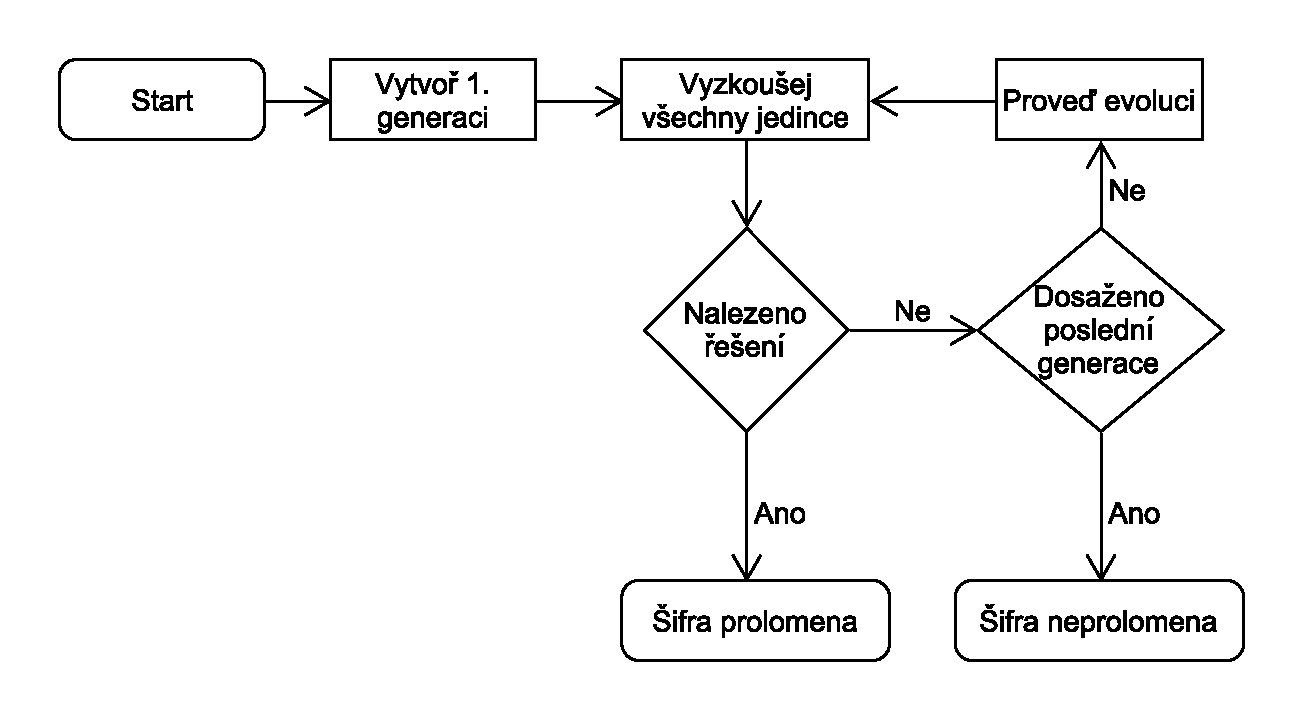
\includegraphics[height=7.5cm]{img/alg-flowchart}
		\caption{Algoritmus řešení}
		\label{fig:alg}
	\end{figure}
	
	\subsection{Diferenciální evoluce}
	Diferenciální evoluce je v principu velmi podobná klasickým genetickým algoritmům. Liší se od nich počtem rodičů (\textgreater2) potřebným k tvorbě potomka a pořadím operací mutace, křížení \cite{hlavacek_de}. 
	
	Při evoluci jedince se nejprve mutací získá šumový vektor, který se pak zkříží s aktivním jedincem (právě zpracovávaný jedinec v generaci). Pokud má takto vzniklý jedinec lepší skóre než aktivní, použije se do nové populace. Evoluce je řízena dvěma parametry: mutační konstantou \textit{F} a prahem křížení \textit{CR}. Doporučené hodnoty jsou 0,3 -- 0,9 pro \textit{F} a 0,8 -- 0,9 pro \textit{CR} \cite{hlavacek_de}. Hodnoty použité v mém řešení jsou uvedeny v tabulce \ref{tab:param-val}.
	
	\begin{table}[H]
		\begin{center}	
			\begin{tabular}{|c|c|}
				\hline
				Parametr & Hodnota \\
				\hline
				\hline
				F & 0,3 \\
				\hline
				CR & 0,5 \\
				\hline 
				Velikost populace & 4160 \\
				\hline
				Maximální počet generací & 1000 - 2000 \\
				\hline
			\end{tabular}
		\end{center}
		\caption{Hodnoty parametrů evoluce}
		\label{tab:param-val}
	\end{table}
	
	V algoritmu diferenciální evoluce je možné použít několik mutačních funkcí \cite{hlavacek_de}, na doporučení vyučujícího jsem použil mutační funkci \textit{best/2}. Ta je znázorněna v rovnici \ref{eq:best2}, $v_{best}$ je nejlepší jedinec v současné generaci, $v_1,v_2,v_3,v_4$ jsou náhodně vybraní, nestejní jedinci (pro každého aktivního jedince jsou vybráni znovu) a F je výše zmíněná mutační konstanta. Výsledkem mutace je šumový vektor $noise$. 
	
	\begin{equation}
		noise = v_{best} + F\cdot(v_1+v_2-v_3-v_4)
		\label{eq:best2}
	\end{equation}
	
		Šumový vektor je následně zkřížen (binomické křížení) s aktivním jedincem a pokud je výsledný vektor lepší než aktivní jedinec, použije se v nové generaci.
	
	\subsubsection{Cenová funkce}
	Jako cenovou funkci jsem použil variantu Hammingovo vzdálenosti dešifrovaného bloku od bloku referečního. Během implementace jsem experimentoval s více cenovými funkcemi a držel jsem se konvence větší skóre znamená lepšího jedince. U Hammingovo vzdálenosti to ale neplatí, proto jsem tuto vzdálenost odečetl od maximální možné vzdálenosti (viz rovnice \ref{eq:fitness}).
	
	\begin{equation}
		fitness = D_{max} - D(decrypted,reference)
		\label{eq:fitness}
	\end{equation}
	
	Tato cenová funkce nekonverguje, vzhledem k povaze šifry SkipJack, příliš dobře, jak je vidět na obrázku \ref{fig:fitness-chart}. Během přednášek nám byla vyučujícím doporučena dvojrozměrná cenová funkce, tu se mi bohužel nepodařilo funkčně naimplementovat.
	
	\begin{figure}[!h]
		\centering
		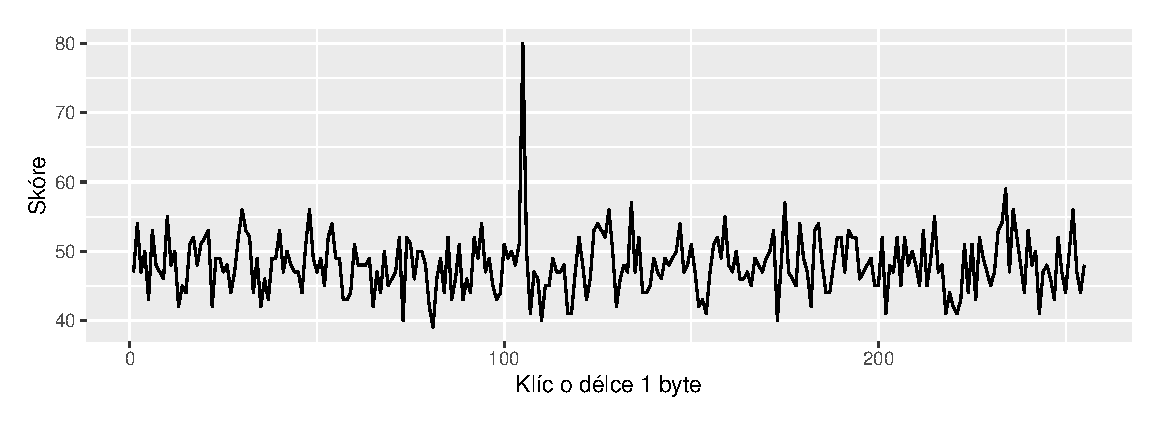
\includegraphics[width=15cm]{img/fitness-plot}
		\caption{Hodnoty fitness funkce pro klíč délky 1}
		\label{fig:fitness-chart}
	\end{figure}

	Kromě Hammingovo vzdálenosti dešifrovaného bloku od referenčního jsem experimentoval i se vzdáleností jedince od referenčního hesla. V tomto případě algoritmus konverguje dobře (100-200 generací), nicméně znalost hesla není běžný případ a proto jsem tuto cenovou funkci použil pouze k odstranění chyb v implementaci evolučního algoritmu.
	
	
	\subsection{Paralelizace}
	Výpočetně nejnáročnější část algoritmu je (kromě fitness funkce, která vytváří klíč a dešifruje) mutační funkce. Proto jsem s paralelizací začal právě v tomto místě. K tomu jsem postupně využil tři technologie: vektorové instrukce, knihovnu Intel TBB a knihovnu OpenCL. 
	
	\paragraph{Vektorové instrukce} Procesor v mém počítači podporuje vektorové instrukce SSE 2 a nižší. Tyto instrukce využívájí vektor délky 128 bitů. Do tohoto vektoru se vejde 16 bytů, což by při maximální délce hesla 10 bytů bylo dostačující, nicméně mutace \textit{best-2} vyžaduje násobení floatem. Nejmenší float, který lze do vektoru uložit zabírá 32 bitů, do vektoru se tedy vejdou jen 3. Aby bylo možné vektorové instrukce v mutační funkci použít, je tedy nutné každý 1 byte hesla roztáhnout na 32 bitů, provést potřebné operace a poté jej z 32 bitů převézt zpátky na 8 bitů. Tato nadbytečná režie způsobila neefektivnost vektorových instrukcí a proto jsem je v mutační funkci nakonec nepoužil.

	\subsubsection{Intel TBB}
	Intel TBB je knihovna pro jazyk C++ sloužící k paralelizacei programů.
	
	NAPSAT LÍP
	
	 Knihovnu jsem použil k paralelizaci evoluce. Původně jsem populaci manuálně rozdělil na dávky, které jsem pak zpracovával pomocí \textit{parallel\_for()}. Tento přístup se ukázal jako neefektivní, protože rozdělení dat mezi vlákny zvládá knihovna sama (a lépe). Proto jsem nakonec logiku evoluce jedince přesunul do funktoru, který následně předávám do \textit{parallel\_for()}.
	
	\subsubsection{OpenCL}
	OpenCL slouží mimojiné k paralelizaci výpočtů pomocí CPU, nebo GPU. Výpočet probíhá v tzv. kernelu, což je funkce napsaná v jazyce OpenCL a přeložená pro dané výpočetní zařízení. Parametry funkce jsou typicky ukazatele na pole s daty z nichž kernel vybere jeden 'řádek' nad kterým provede operaci.
	
	V mém řešení jsem do kernelu přenesl mutaci a křížení jednoho bytu hesla -- kernel je znázorněný na obrázku \ref{fig:kernel}. V kroku evoluce se tedy nejprve nagenerují potřebná data pro celou populaci (pole s vektory $v1$,$v2$,$v3$,$v4$ a pole $randoms$ s náhodnými čísly pro křížení), nad nimi proběhne paralelizovaný výpočet evoluce a nakonec jsou z výsledků vybráni jedinci, kteří přežijí do následující generace. 
	
	\begin{figure}[H]
		\centering
		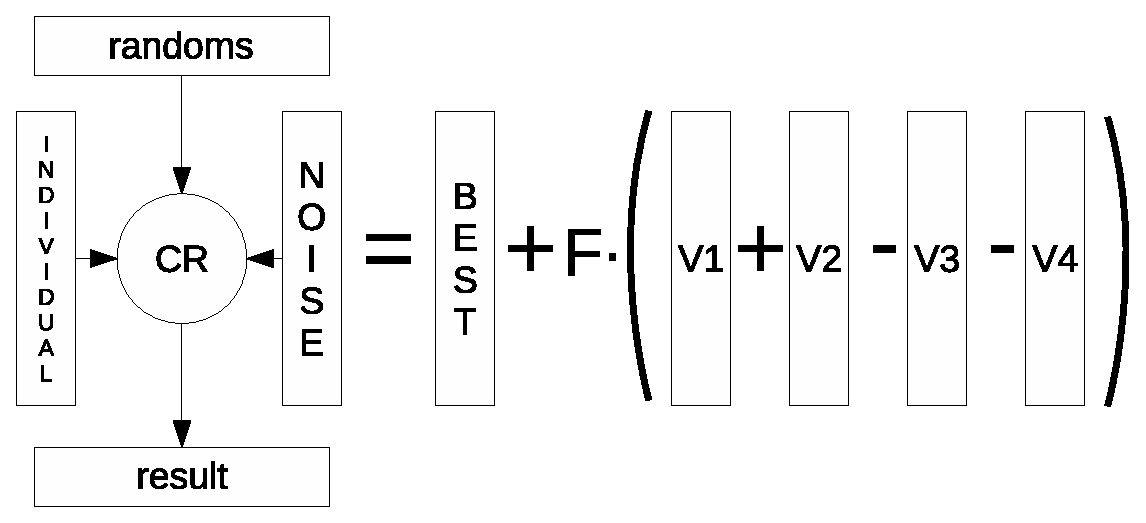
\includegraphics[width=12cm]{img/opencl-data-diag}
		\caption{Operace prováděná v kernelu}
		\label{fig:kernel}
	\end{figure}

	Kvůli nutnosti předpřipravit všechna data před začátkem výpočtu zabírá program při použití OpenCL velké množství paměti -- pole s vektory a náhodnými čísly zabírají téměř 2 MB. V mém počítači mám bohužel jen intergrovanou grafickou kartu ...
	
	\section{Výsledky}
	\label{sec:results}
	Všechna testování jsem prováděl na svém počítači jehož specifikace jsou uvedeny v tabulce \ref{tab:pc-spec}. Pro různá nastavení populace a způsobu zpracování jsem program nechal proběhnout dvacetkrát. Výsledky získané měřením jsou uvedeny v tabulkách \ref{tab:res-serial}, \ref{tab:res-tbb} a \ref{tab:res-opencl}. Měření bylo prováděno s délkou hesla 10 bytů. Šifru se podařilo prolomit pouze při snížení délky hesla na 1 byte.
	
	\begin{table}[H]
		\begin{center}
			\begin{tabular}{|c|c|}
				\hline
				Parametr & Hodnota \\
				\hline
				\hline
				CPU & Intel Pentium B970, 2 jádra, 2,30 GHz, 2MB L3 Cache\\
				\hline
				GPU & integrovaná \\
				\hline
				RAM & 8 GB \\
				\hline
				OS & Windows 7 Ultimate SP 1 \\
				\hline
			\end{tabular}
		\end{center}
		\caption{Specifikace počítače}
		\label{tab:pc-spec}
	\end{table}

	\begin{table}[H]
		\begin{center}
			\begin{tabular}{|c|c|c|}
				\hline
				Počet generací & Průměrná doba běhu [s] & Skóre nejlepšího jedince\\
				\hline
				\hline
				1000 & 12,457 & 54 \\
				\hline
				1500 & 18,589 & 54 \\
				\hline
				2000 & 24,774 & 52 \\
				\hline
			\end{tabular}
		\end{center}
		\caption{Tabulka s výsledky pro běh bez paralelizace}
		\label{tab:res-serial}
	\end{table}

	\begin{table}[H]
		\begin{center}
			\begin{tabular}{|c|c|c|}
				\hline
				Počet generací & Průměrná doba běhu [s] & Skóre nejlepšího jedince\\
				\hline
				\hline
				1000 & 6,825 & 53 \\
				\hline
				1500 & 10,238 & 53 \\
				\hline
				2000 & 13,611 & 52 \\
				\hline
			\end{tabular}
		\end{center}
		\caption{Tabulka s výsledky pro běh s paralelizací knihovnou Intel TBB}
		\label{tab:res-tbb}
	\end{table}

	\begin{table}[H]
		\begin{center}
			\begin{tabular}{|c|c|c|}
				\hline
				Počet generací & Průměrná doba běhu [s] & Skóre nejlepšího jedince\\
				\hline
				\hline
				1000 & 13,111 & 52 \\
				\hline
				1500 & 19,5305 & 54 \\
				\hline
				2000 & 25,923 & 50 \\
				\hline
			\end{tabular}
		\end{center}
		\caption{Tabulka s výsledky pro běh s paralelizací knihovnou OpenCL}
		\label{tab:res-opencl}
	\end{table}

	Z měření vyplývá, že největšího urychlení bylo dosaženo použitím knihovny Intel TBB. Oproti tomu použití knihovny OpenCL program v podstatě neurychlilo, což může být způsobeno špatnou implementací programu, nebo použitím na nevhnodnou část výpočtu.

	\section{Uživatelská příručka}
	Program lze přeložit a sestavit pomocí standardního C/C++ překladače (gcc, cl).
	
	Při sestavení musí mít linker přístup k tbb a opencl. 
	
	Použití: program.exe ref enc 
	
	Pro vyzkoušení s/bez paralelizmu nutné překompilovat.
	

	
	\section{Závěr}
	Šifru se nepodařilo prolomit, vyzkoušel jsem si paralelizaci, OpenCL se mi nepodařilo naimplementovat tak, aby to zrychlovalo.
	
	\begin{thebibliography}{9}
		\bibitem{hlavacek_de}
		HLAVÁČEK, Jiří. \textit{Moderní adaptivní diferenciální evoluce} [online]. Zlín, 2015 [cit. 2018-11-22]. Dostupné z: \textless https://theses.cz/id/vs0ow2/\textgreater. Diplomová práce. Univerzita Tomáše Bati ve Zlíně, Fakulta aplikované informatiky. Vedoucí práce doc. Ing. Roman Šenkeřík, Ph.D
	\end{thebibliography}
	
\end{document}
